\documentclass[journal,12pt,twocolumn]{IEEEtran}

\usepackage{setspace}
%\usepackage{gensymb}
\singlespacing
\usepackage[cmex10]{amsmath}

\usepackage{amsthm}

\usepackage{mathrsfs}
\usepackage{txfonts}
%\usepackage{stfloats}
\usepackage{bm}
\usepackage{cite}
%\usepackage{cases}
\usepackage{subfig}

\usepackage{longtable}
%\usepackage{multirow}

%\usepackage{enumitem}
\usepackage{mathtools}
%\usepackage{steinmetz}
%\usepackage{tikz}
%\usepackage{circuitikz}
\usepackage{verbatim}
%\usepackage{tfrupee}
\usepackage[breaklinks=true]{hyperref}
\usepackage{graphicx}
%\usepackage{tkz-euclide}

%\usetikzlibrary{calc,math}
\usepackage{listings}
    \usepackage{color}                                            %%
    \usepackage{array}                                            %%
    \usepackage{longtable}                                        %%
    \usepackage{calc}                                             %%
    %\usepackage{multirow}                                         %%
    \usepackage{hhline}                                           %%
    \usepackage{ifthen}                                           %%
    \usepackage{lscape}     
\usepackage{multicol}
%\usepackage{chngcntr}

\DeclareMathOperator*{\Res}{Res}

\renewcommand\thesection{\arabic{section}}
\renewcommand\thesubsection{\thesection.\arabic{subsection}}
\renewcommand\thesubsubsection{\thesubsection.\arabic{subsubsection}}

\renewcommand\thesectiondis{\arabic{section}}
\renewcommand\thesubsectiondis{\thesectiondis.\arabic{subsection}}
\renewcommand\thesubsubsectiondis{\thesubsectiondis.\arabic{subsubsection}}


\hyphenation{op-tical net-works semi-conduc-tor}
\def\inputGnumericTable{}                                 %%

\lstset{
%language=C,
frame=single, 
breaklines=true,
columns=fullflexible
}
\begin{document}


\newtheorem{theorem}{Theorem}[section]
\newtheorem{problem}{Problem}
\newtheorem{proposition}{Proposition}[section]
\newtheorem{lemma}{Lemma}[section]
\newtheorem{corollary}[theorem]{Corollary}
\newtheorem{example}{Example}[section]
\newtheorem{definition}[problem]{Definition}

\newcommand{\BEQA}{\begin{eqnarray}}
\newcommand{\EEQA}{\end{eqnarray}}
\newcommand{\define}{\stackrel{\triangle}{=}}
\bibliographystyle{IEEEtran}
\raggedbottom
\setlength{\parindent}{0pt}
\providecommand{\mbf}{\mathbf}
\providecommand{\pr}[1]{\ensuremath{\Pr\left(#1\right)}}
\providecommand{\qfunc}[1]{\ensuremath{Q\left(#1\right)}}
\providecommand{\sbrak}[1]{\ensuremath{{}\left[#1\right]}}
\providecommand{\lsbrak}[1]{\ensuremath{{}\left[#1\right.}}
\providecommand{\rsbrak}[1]{\ensuremath{{}\left.#1\right]}}
\providecommand{\brak}[1]{\ensuremath{\left(#1\right)}}
\providecommand{\lbrak}[1]{\ensuremath{\left(#1\right.}}
\providecommand{\rbrak}[1]{\ensuremath{\left.#1\right)}}
\providecommand{\cbrak}[1]{\ensuremath{\left\{#1\right\}}}
\providecommand{\lcbrak}[1]{\ensuremath{\left\{#1\right.}}
\providecommand{\rcbrak}[1]{\ensuremath{\left.#1\right\}}}
\theoremstyle{remark}
\newtheorem{rem}{Remark}
\newcommand{\sgn}{\mathop{\mathrm{sgn}}}
\providecommand{\abs}[1]{\left\vert#1\right\vert}
\providecommand{\res}[1]{\Res\displaylimits_{#1}} 
\providecommand{\norm}[1]{\left\lVert#1\right\rVert}
%\providecommand{\norm}[1]{\lVert#1\rVert}
\providecommand{\mtx}[1]{\mathbf{#1}}
\providecommand{\mean}[1]{E\left[ #1 \right]}
\providecommand{\fourier}{\overset{\mathcal{F}}{ \rightleftharpoons}}
%\providecommand{\hilbert}{\overset{\mathcal{H}}{ \rightleftharpoons}}
\providecommand{\system}{\overset{\mathcal{H}}{ \longleftrightarrow}}
	%\newcommand{\solution}[2]{\textbf{Solution:}{#1}}
\newcommand{\solution}{\noindent \textbf{Solution: }}
\newcommand{\cosec}{\,\text{cosec}\,}
\providecommand{\dec}[2]{\ensuremath{\overset{#1}{\underset{#2}{\gtrless}}}}
\newcommand{\myvec}[1]{\ensuremath{\begin{pmatrix}#1\end{pmatrix}}}
\newcommand{\mydet}[1]{\ensuremath{\begin{vmatrix}#1\end{vmatrix}}}
\numberwithin{equation}{subsection}
\makeatletter
\@addtoreset{figure}{problem}
\makeatother
\let\StandardTheFigure\thefigure
\let\vec\mathbf
\renewcommand{\thefigure}{\theproblem}
\def\putbox#1#2#3{\makebox[0in][l]{\makebox[#1][l]{}\raisebox{\baselineskip}[0in][0in]{\raisebox{#2}[0in][0in]{#3}}}}
     \def\rightbox#1{\makebox[0in][r]{#1}}
     \def\centbox#1{\makebox[0in]{#1}}
     \def\topbox#1{\raisebox{-\baselineskip}[0in][0in]{#1}}
     \def\midbox#1{\raisebox{-0.5\baselineskip}[0in][0in]{#1}}
\vspace{3cm}
\title{EE3025 Assignment-1}
\author{Yuvateja - EE18BTECH11043}
\maketitle
\bigskip
\renewcommand{\thefigure}{\theenumi}
\renewcommand{\thetable}{\theenumi}
\bigskip
Download all python codes from 
\begin{lstlisting}
https://github.com/yuvateja-ctrl/EE3025/tree/main/codes
\end{lstlisting}



%
and latex-tikz codes from 
%
\begin{lstlisting}
https://github.com/yuvateja-ctrl/EE3025
\end{lstlisting}
\section{Digital Filter}
1.1 Download the sound file from  
\begin{lstlisting}
wget https://raw.githubusercontent.com/gadepall/ 
EE1310/master/filter/codes/Sound_Noise.wav
\end{lstlisting}
1.2 Write the python code for removal of out of band noise and execute the code.
\\
\solution
\lstinputlisting{./codes/cancel_noise.py}
\section{Difference equation}
2.1 Write the difference equation of above Digital filter obtained in problem 1.2.
\\
\solution
\begin{equation}
\label{eq:iir_filter_gen}
 \sum _{m=0}^{M}a\brak{m}y\brak{n-m}=\sum _{k=0}^{N}b\brak{k}x\brak{n-k}
\end{equation}
\begin{equation}
\label{eq:diff_eqn}
\begin{split}
y(n) - 2.52y(n-1) + 2.56y(n-2) - 1.206y(n-3)
\\
+ 0.22013y(n-4) = 0.00345x(n) + 0.0138x(n-1) +
\\
 0.020725x(n-2) + 0.0138x(n-3) + 0.00345x(n-4)
\end{split}
\end{equation}

2.2 Sketch x(n) and y(n).
\\
\solution
The following code yields Fig 2.2
\begin{lstlisting}
codes/inp_out.py
\end{lstlisting}
The filtered sound signal obtained through difference equation is found in
\begin{lstlisting}
codes/Sound_de.wav
\end{lstlisting}
\begin{figure}[!ht]
\begin{center}
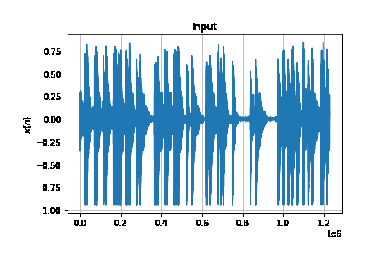
\includegraphics[width=8cm]{./figs/input.eps}
\end{center}
\captionof{figure}{}
\label{fig:Input}	
\end{figure}
\begin{figure}[!ht]
\begin{center}
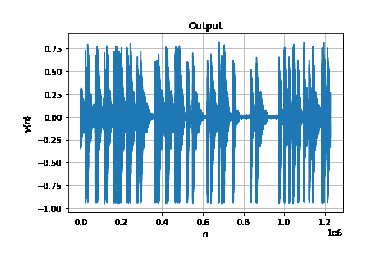
\includegraphics[width=8cm]{./figs/output.eps}
\end{center}
\captionof{figure}{}
\label{fig:Input}	
\end{figure}
\section{Z-transform}

\label{prob:Z-transform_formula}
%
3.1
\begin{equation}
\label{eq:z_trans}
X(z)={\mathcal {Z}}\{x(n)\}=\sum _{n=-\infty }^{\infty }x(n)z^{-n}
\end{equation}
%
Show that
\begin{equation}
\label{eq:shift1}
{\mathcal {Z}}\{x(n-1)\} = z^{-1}X(z)
\end{equation}
and find
\begin{equation}
	{\mathcal {Z}}\{x(n-k)\} 
\end{equation}
\\
\solution From 3.0.1,
\begin{align}
{\mathcal {Z}}\{x(n-k)\} &=\sum _{n=-\infty }^{\infty }x(n-1)z^{-n}
\\
&=\sum _{n=-\infty }^{\infty }x(n)z^{-n-1} = z^{-1}\sum _{n=-\infty }^{\infty }x(n)z^{-n}
\end{align}
resulting in 3.0.2. Similarly, it can be shown that
%
\begin{equation}
\label{eq:z_trans_shift}
	{\mathcal {Z}}\{x(n-k)\} = z^{-k}X(z)
\end{equation}
Find
%
\begin{equation}
H(z) = \frac{Y(z)}{X(z)}
\end{equation}
%
from  2.0.2 assuming that the $Z$-transform is a linear operation.
\\
\solution  Applying 3.0.6 in 2.0.2 we get,
\begin{equation}
\begin{split}
H(z) = \frac{Y(z)}{H(z)}                
\\
=\frac{b[0]+b[1]z^{-1}+b[2]z^{-2}+b[3]z^{-3}+b[4]z^{-4}}{a[0]+a[1]z^{-1}+a[2]z^{-2}+a[3]z^{-3}+a[4]z^{-4}}
\label{eq:freq_resp}
\end{split}
\end{equation}
%
Let
\begin{equation}
H\brak{e^{\j w}} = H\brak{z = e^{\j w}}.
\end{equation}
Plot $\abs{H\brak{e^{\j w}}}$.
\\
\solution
The following code plots Fig 3.3.
\begin{lstlisting}
codes/dtft.py
\end{lstlisting}
\begin{figure}[!ht]
\centering
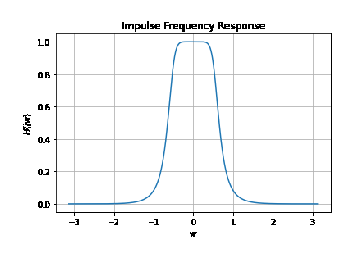
\includegraphics[width=8cm]{./figs/impulse_response.eps}
\caption{$\abs{H\brak{e^{\j w}}}$}
\label{fig:H(jw)}
\end{figure}
\section{Impulse Response}
4.1 From the difference equation eq. 2.0.2. Sketch h(n)
\label{prob:h(n)}
\\
\solution
we know that output would be impulse response when the given input is impulse. 
From 2.0.1, \\
By substituting $x(n-k) = \delta(n-k)$, then $y(n-k)$ becomes $h(n-k)$ for all k=0,1,2,3,4.
Now, the following code plots Fig 4.1
\begin{lstlisting}
codes/impulseRes_def.py
\end{lstlisting}
\begin{figure}[!ht]
\centering
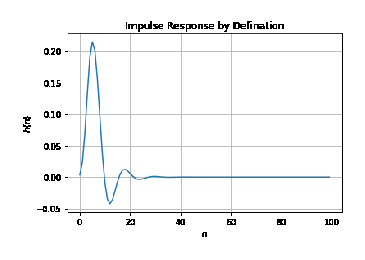
\includegraphics[width=8cm]{./figs/impy_def.eps}
\caption{$h(n)$}
\label{fig:h(n)}
\end{figure}
4.2 Check whether h(n) obtained is stable.
\\
\solution
The system is defined by the equation 2.0.2 \\
By BIBO(Bounded Input Bounded Output) we know that if the input is bounded then the output should also be bounded.

Since x(n) is bounded, let $B_{x}$ be some finite value
\begin{equation}
\abs{y(n)} \leq B_{x}\sum_{-\infty}^{\infty} \abs{x(n-k)}
\end{equation}
From convolution formula,
\begin{equation}
\abs{y(n)} = \abs{\sum_{-\infty}^{\infty} h(k)x(n-k)}
\end{equation}
\begin{equation}
\abs{y(n)} \leq \sum_{-\infty}^{\infty} \abs{h(k)}\abs{x(n-k)}
\end{equation}
Let $B_{x}$ be the maximum value x(n-k) can take, then
\begin{equation}
\abs{y(n)} \leq B_{x}\sum_{-\infty}^{\infty} \abs{h(k)}
\end{equation}
If
\begin{equation}
\sum_{-\infty}^{\infty} \abs{h(k)} < \infty
\end{equation}
Then
\begin{equation}
\abs{y(n)} \leq B_{y} < \infty
\end{equation}
Hence y(n) is bounded if both input x(n) and system tranfer function h(n) are bounded.\\
Here as audio input is also bounded we can say the system is said to be stable.
\begin{equation}
\sum_{n=-\infty}^{n=-\infty} \abs{h(n)}<\infty
\end{equation}
The above euation can be re written as,
\begin{equation}
\sum_{n=-\infty}^{n=-\infty} \abs{h(n)z^{-n}}_{\abs{z}=1}<\infty
\end{equation}
\begin{equation}
\sum_{n=-\infty}^{n=-\infty} \abs{h(n)} \abs{z^{-n}}_{\abs{z}=1}<\infty
\end{equation}
From Triangle inequality,
\begin{equation}
\abs{\sum_{n=-\infty}^{n=-\infty} h(n)z^{-n}}_{\abs{z}=1}<\infty
\end{equation}
\begin{equation}
\implies \abs{H(n)}_{\abs{z}=1} < \infty
\end{equation}
Therefore, the Region of Convergence(ROC) should include the unit circle for the system to be stable.
Since, h(n) is right sided the ROC is outside the outer most pole. From the equation 3.0.8
Poles of the given transfer equation is:
\begin{equation}
\begin{split}
z(approx) = 0.69382 \pm 0.41i,
\\
 0.56617835 \pm 0.134423
\end{split}  
\end{equation}
From the above poles, we can see that that the ROC of the system is $\abs{z}>\sqrt{0.69382^{2}+0.41^{2}}$.
\begin{figure}[!ht]
\centering
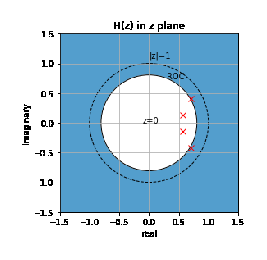
\includegraphics[width=6cm]{./figs/roc.eps}
\caption{ROC plot}
\label{fig:xnhnfft}
\end{figure}
From the figure we can observe that ROC of the system includes unit circle $\abs{z}=1$.
The code for plotting the figure is:
\begin{lstlisting}
    codes/roc.py
\end{lstlisting}
Which implies that the given IIR filter is stable, because h(n) is absolutely summable.And the given system is stable.

4.3 Compute Filtered output using convolution formula using h(n) obtained in 4.1
%
\begin{equation}
\label{eq:convolution}
y(n) = x(n)*h(n) = \sum_{n=-\infty}^{\infty}x(k)h(n-k)
\end{equation}
\solution The following code plots Fig 4.3
%
\begin{lstlisting}
/codes/out_conv.py
\end{lstlisting}
\begin{figure}[!ht]
\centering
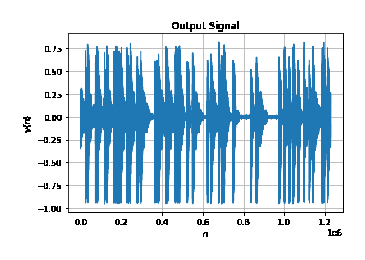
\includegraphics[width=8cm]{./figs/digital_filter_output.eps}
\caption{$y(n)$ from the definition of convolution}
\label{fig:yn_conv}
\end{figure}
The filtered sound signal through convolution from this method is found in
\begin{lstlisting}
codes/Sound_conv.wav
\end{lstlisting}
We can observe that the output obtained is same as y(n) obtained in Fig 2.2
\section{FFT and IFFT}
5.1 compute
\begin{align}
        X(k) \triangleq \sum_{n=0}^{N-1} x(n) e^{-j 2 \pi k n / N}, \quad k=0,1, \ldots, N-1
\end{align}
and $H(k)$ using h(n).
\\
\solution
For this given IIR system with audio sample as x(n) and h(n) as impulse response h(n) obtained in 4.1 
DFT of a Input Signal $x(n)$ is 
\begin{align}
    X(k) \triangleq \sum_{n=0}^{N-1} x(n) e^{-j 2 \pi k n / N}, \quad k=0,1, \ldots, N-1
\end{align}
DFT of a Impulse Response $h(n)$ is 
\begin{align}
    H(k) \triangleq \sum_{n=0}^{N-1} h(n) e^{-j 2 \pi k n / N}, \quad k=0,1, \ldots, N-1
\end{align}
The following code plots FFT of $x(n)$ and $h(n)$.
\begin{lstlisting}
    codes/xn_hn_fft.py
\end{lstlisting}
Magnitude and Phase plots obtained through above code is\\ 
\begin{figure}[!ht]
\centering
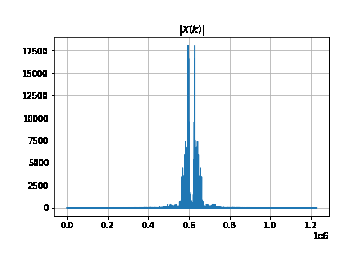
\includegraphics[width=8cm]{./figs/abs_xk.eps}
\caption{Magnitude of X(k)}
\label{fig:xfft}
\end{figure}
\begin{figure}[!ht]
\centering
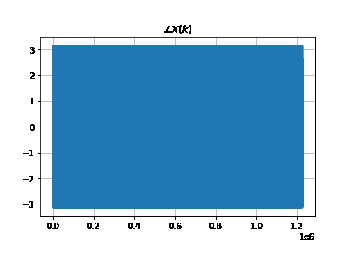
\includegraphics[width=9cm]{./figs/phase_xk.eps}
\caption{Phase of X(k)}
\label{fig:xfft}
\end{figure}
\begin{figure}[!ht]
\centering
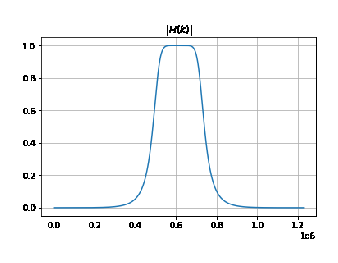
\includegraphics[width=10cm]{./figs/abs_hx.eps}
\caption{Magnitude of H(k)}
\label{fig:hfft}
\end{figure}
\newpage
\begin{figure}[!ht]
\centering
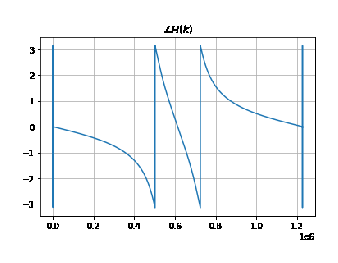
\includegraphics[width=8cm]{./figs/phase_hx.eps}
\caption{Phase of H(k)}
\label{fig:hfft}
\end{figure}
5.2 From
\begin{equation}
Y(k) = X(k)H(k)
\end{equation}
Compute
\begin{equation}
y(n) \triangleq \sum_{k=0}^{N-1} Y(k) e^{j 2 \pi k n / N}, \quad n=0,1, \ldots, N-1
\end{equation}
\\
\solution
\\The following code plots Fig 5.2
\begin{lstlisting}
    codes/out_fft.py
\end{lstlisting}
\begin{figure}[!ht]
\centering
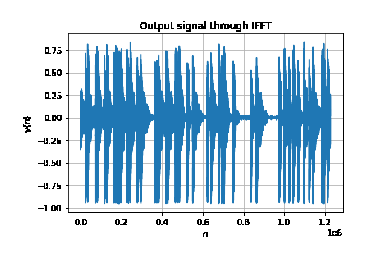
\includegraphics[width=9cm]{./figs/output_ifft.eps}
\caption{$y(n)$}
\label{fig:ynfft}
\end{figure}
\newpage
The filtered sound signal from this method is found in
\begin{lstlisting}
codes/Sound_fft.wav
\end{lstlisting}
We can observe from the above plot that it is same as the y(n) observed in Fig 2.2
\end{document}
